\documentclass[english,letter,11pt,twoside]{article}

\usepackage{basilestyle2}
\usepackage[bottom]{footmisc}
\usepackage{ae,aecompl}
\usepackage[english]{babel}
\usepackage{amsmath}
\usepackage{amsfonts}
\usepackage{amssymb}
\usepackage{booktabs,subfigure}
\usepackage{comment}
\usepackage{mathtools}
%Some command to parametrize the marginal
\geometry{vmargin=2.4cm,hmargin=2.6cm}

%the paragraph space
\setlength{\parindent}{0pt} 
%\setlength{\parskip}{1ex plus 4.ex minus .2ex}

%The space between lines
\linespread{1.2}


\usepackage{colortbl}
%to use the command multi row in tables
\usepackage{multirow}

%three part table
\usepackage[flushleft]{threeparttable}

%multi columns table
\usepackage{multicol}
\setlength{\columnsep}{1cm}

%better tabulate and line in tables
\usepackage{booktabs}


%some colors
\def\tcr{\textcolor{red}}
\def\tcb{\textcolor{blue}}
\def\tcp{\textcolor{purple}}
\def\rc{\textcolor{blue}{rc edits}}

\title{\Large Replication: Distorsions in Production Networks \\
\large by Jennifer La'O and Saki Bigio, QJE 2020}
\author{Piero De Dominicis}
\date{\normalsize \today}

\begin{document}
\maketitle


The baseline model presented in the paper has a CRS technology structure and a single primary factor of labor. In the quantitative application they relax this assumption modifying the production function as follows:
\begin{align*}
	y_{it} = z_{i,t} \left( \ell_{i,t}^{\alpha_i} x_{i,t}^{1- \alpha_i} \right)^{\eta_i}
\end{align*}
where $\eta_i \in \left(0,1\right]$ controls for the sector's specific DRS and $x_{i,t} = \prod_{j = 1}^{N} x_{ij,t}^{g_{ij}}$ are the purchases of sectoral commodity $j$ from firm $i$. The coefficients $g_{ij}$ are calibrated using BEA input-output tables, specifically $g_{ij} = \frac{p_{ij x_{ij,t}}}{\sum_j p_{jt} x_{ij,t}}$. Similarly, $\alpha_i$ are calibrated using labor expenses in sector $i$: $\frac{W_t \ell_{it}}{W_t \ell_{it} + \sum_j p_{jt} x_{ij,t}}$. These parameters have been particularly stable over the years, therefore for the quantitative exercise the model is calibrated using 2007 values only and then simulated for the periods following the financial crisis.



The main quantitative exercise of the paper is to investigate what is the role played by the input-output network in amplifying the financial frictions documented by \cite{gilchrist2012credit}. To answer this question, they compare the calibrated network model to an equivalent model in which I-O linkages are absent, such that all sectors sell their output directly to the household. To quantify the importance of I-O in amplifying these distorsions, they define:
\begin{itemize}
	\item the \textit{labor wedge network multiplier}: the ratio between the percentage change in the labor wedge generated by the I-O economy and the one generated by the horizontal economy;
	\item the \textit{TFP network multiplier}: the ratio between the percentage change in the TFP wedge generated by the I-O economy and the one generated by the horizontal economy.
\end{itemize}

The authors offer a reinterpretation of sectoral distorsions as financial frictions by introducing withing-period financing decisions. The intermediate firms must pay all working-capital costs at the beginning of the period. Therefore, firms must ask for a loan in order to finance the purchase of the inputs used for production.
The financial frictions of \cite{gilchrist2012credit} is defined as:
\begin{align*}
\phi_{it} = \frac{1}{1 + r_{it}^{GZ}}
\end{align*}
where $r_{it}^{GZ}$ are sector-level indices which can be interpreted as excess bond premia. The GZ excess bond premium can be interpreted as the intraperiod borrowing rate faced by sector $i$ in period $t$. Next, we define symmetric and asymmetric distorsions and explain how they are used in the quantitative exercise.

\paragraph*{Symmetric Distorsions} First, they simulate the two alternative economies for 2008-2009 by feeding symmetric distorsions to the model. Symmetric distorsions are computed using the mean of $\Delta \log \phi_{it}$ during the same period. The \textit{labor wedge multiplier} is computed using symmetric distorsions in order to isolate the role of the network structure in amplifying distorsions.

\paragraph*{Asymmetric Distorsions} Second, they simulate the two economies by feeding asymmetric distorsions to the model. GZ distorsions are very heterogeneous across sectors, it is therefore important to allow for this source of heterogeneity to fully understand how the I-O structure amplify the distorsions in the presence of heterogeneous frictions. 

\paragraph*{The Labor and Efficiency Wedge during the 2008-09 crisis} In Table \ref{Table1}, we report the results of the simulations as the differences between the 2008 and 2009 values.

\begin{table}[h]
\label{Table1}
\begin{center}
  \setlength\extrarowheight{5pt}
    \caption{The Labor Wedge Network Multiplier During the 2008-09 Financial Crisis}
    \vspace*{0.2cm}
\scalebox{1}{%
\begin{tabular}{ccccc}
\hline \hline
& \multicolumn{2}{c}{$\Delta \log A$}  & \multicolumn{2}{c}{$\Delta \log \Lambda$}  \\
Returns to scale & DRS & CRS & DRS & CRS \\ \hline
Horizontal, symmetric $\phi $& $0$ & $0$ & $-0.0307$ & $-0.0307$ \\
U.S. IO network, symmetric $\phi$ & $-0.0012$ & $-0.0027$ & $-0.0523$ & $-0.0650$ \\
U.S. IO network, asymmetric $\phi$ & $-0.0013$ & $-0.0028$ & $-0.0493$ & $-0.0591$ \\
Network Multiplier & $\infty$ & $\infty$ & $1.70$ & $2.12$ \\
\hline \hline
\end{tabular}}
 \end{center}
 
\begin{center}
{\parbox{5.5in}{
\footnotesize Note: The network multiplier is calculated as the ratio between the second and the first line. $\Delta \log A$ and $\Delta \log \Lambda$ are differences between 2008 and 2009 values.
}}
\end{center}
\end{table}

If we consider an economy without input-output linkages, that is every good is only directly sold to the household instead of being used as intermediate input for production, then the efficiency wedge arise only if sectoral distortions are asymmetric\footnote{If every sector is distorted in the same way, then at aggregate level there are not gonna be any distortions.}.

Table \ref{Table1} shows the changes in the labor and efficiency wedges between 2008 and 2009 obtained from the simulation of the model. In an horizontal economy, symmetric sectoral distorsions do not have any effect on the aggregate efficiency wedge, resulting in a Network Multiplier $\approx \infty$. If we consider instead a Network economy with symmetric distorsions, we have a negative effect on the efficiency wedge, although the magnitude of such change is small. The labor wedge, on the contrary, is also affected in an horizontal economy with symmetric sectoral distortions, and by adding the specific network structure, this effect is amplified. This result suggests that the U.S. Input-Output structure nearly ``doubled'' the macroeconomic effect of financial distorsions during the Great Recession. Next, we graphically show the different impact of distorsions on the labor wedge and on the efficiency wedge. \ref{efficiency_graph} confirms what previously said: in an horizontal economy the impact of symmetric distorsions is null, whereas in an I-O economy with either symmetric or asymmetric distorsions the changes in the efficiency wedge are quantitatively small. 

\begin{figure}[!h]
\centering
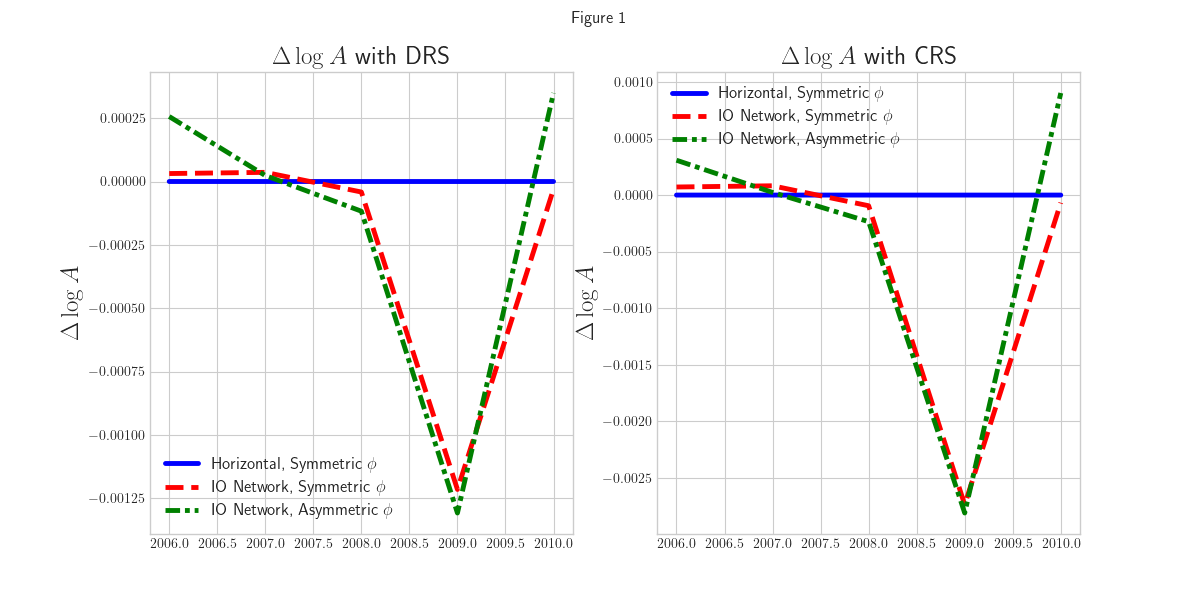
\includegraphics[scale=0.5]{figure1.png}
\caption{The Model-Generated Efficiency Wedge}
\label{efficiency_graph}
\end{figure}

\begin{figure}[!h]
\centering
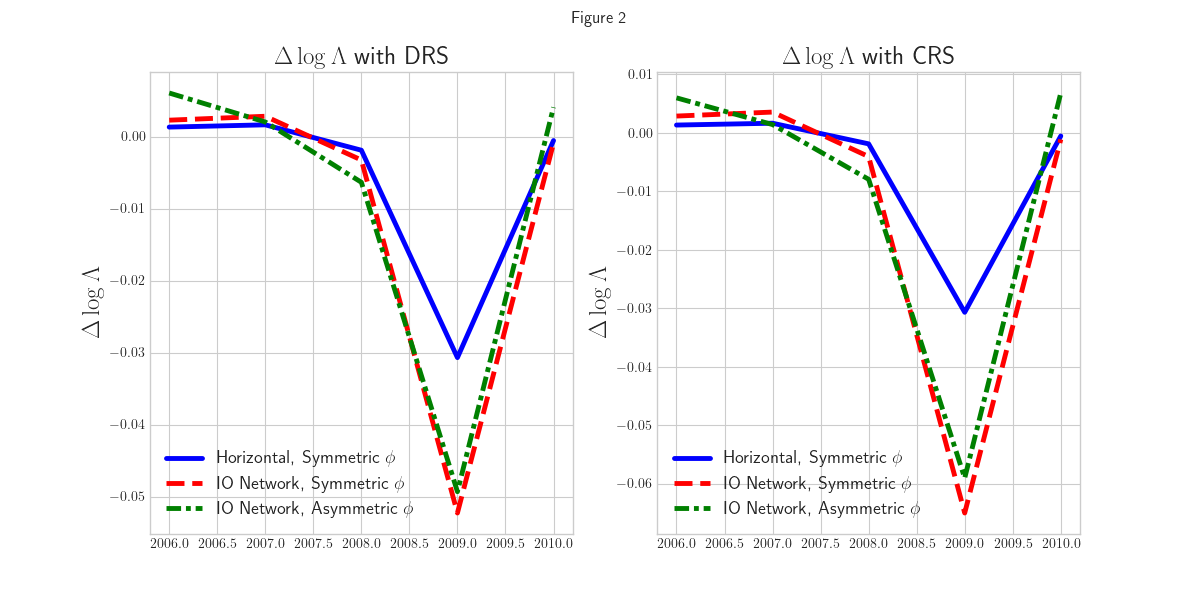
\includegraphics[scale=0.5]{figure2.png}
\caption{The Model-Generated Labor Wedge}
\label{labor_graph}
\end{figure}
In Figure \ref{labor_graph}, we report the model-generated labor wedge. The relative scale compared to Figure \ref{efficiency_graph} is much larger, confirming that financial frictions had a stronger impact on the labor wedge during the financial crisis. 


\paragraph*{Model-Generated Wedges and Data Counterpart:} It is possible to compute the model-implied movements in $\log A(s)$ and $\log \Lambda (s)$ from $1998$ to $2015$. The authors construct a data counterpart for the labor wedge using standard assumption of preferences homotheticity:
\begin{align*}
	U(C) \equiv \frac{C^{1 - \gamma}}{1 - \gamma} \quad \text{and} \quad V(L) \equiv \frac{L^{1+\epsilon}}{1 + \epsilon}
\end{align*} 
where $\epsilon$ is the inverse Frisch elasticity, and $\gamma$ the relative risk aversion parameter.

The above preferences specification results in the following system of equations in two unknowns:
\begin{align*}
L(s)^{\epsilon} &= \Lambda(s) C(s)^{-\gamma} \frac{C(s)}{L(s)} & \forall \ s \in S \\
C(s) &= A(s) L(s) & \forall \ s \in S
\end{align*}
where the first one is the usual intratemporal condition, and the second is a resource constraint $C(s) = Y(s)$. Plugging the second equation in the first we get an expression for aggregate labor:
\begin{align*}
L(s)^{\epsilon + \gamma} &= \Lambda(s) A(s)^{1 - \gamma} & \forall \ s \in S \\
\log L(s) &= \frac{1}{\epsilon + \gamma} \log \Lambda (s) + \frac{1 - \gamma}{\epsilon + \gamma} \log A(s) & \forall \ s \in S
\end{align*}
and substituting back into the second equation we get an expression for aggregate consumption:
\begin{align*}
C(s) &= A(s) L(s) & \forall \ s \in S \\
\log C(s) &= \log A(s) + \log L(s) & \forall \ s \in S \\
\log C(s) &= \log A(s) + \frac{1}{\epsilon + \gamma} \log \Lambda (s) + \frac{1 - \gamma}{\epsilon + \gamma} \log A(s) & \forall \ s \in S \\
\log C(s) &= \frac{1}{\epsilon + \gamma} \log \Lambda (s) + \frac{1 + \epsilon}{\epsilon + \gamma} \log A(s) & \forall \ s \in S 
\end{align*}

From these equations, we can derive the model-generated labor wedge as:
\begin{align*}
\log \Lambda (s) &= \left( 1 + \epsilon \right) \log L(s) - \left( 1 -\gamma \right) \log C(s)
\end{align*}
where we can use data for $L(s)$ and $C(s)$. Finally, they set $\epsilon = 0.5$, implying a Frisch elasticity of labor supply of $2$, and $\gamma = 0.1$. Notice that in this framework, $\gamma$ controls only the elasticity of labor supply to income for a given wage, given that risk aversion and intertemporal substitution play no role as all idiosyncratic risk is uninsurable and the model is static.

Figure \ref{model_wedges} plot the model-implied movements in $\log A(s)$ and $\log \Lambda (s)$ from $1998$ to $2015$. Movements in both the DRS and CRS are similar, with the CRS have just amplified effects in the fluctuations for the two aggregate wedges. The Data counterpart for $\log \Lambda (s)$ are constructed using the derived expression for homothetic preferences 
\begin{align*}
\log \Lambda (s) = \left( 1 + \epsilon \right) \log \hat{L} - \left( 1 -\gamma \right) \log \hat{C} 
\end{align*}
where $\hat{L}$ and $\hat{C}$ are respectively aggregate consumption and hours computed in the data. Fluctuations in the model-implied wedges and data counterpart are very similar, the calibrated network model with GZ shocks can account for 73-88\% of the fall in the labor wedge computed in our data from 2008-2009.


\begin{figure}[!h]
\centering
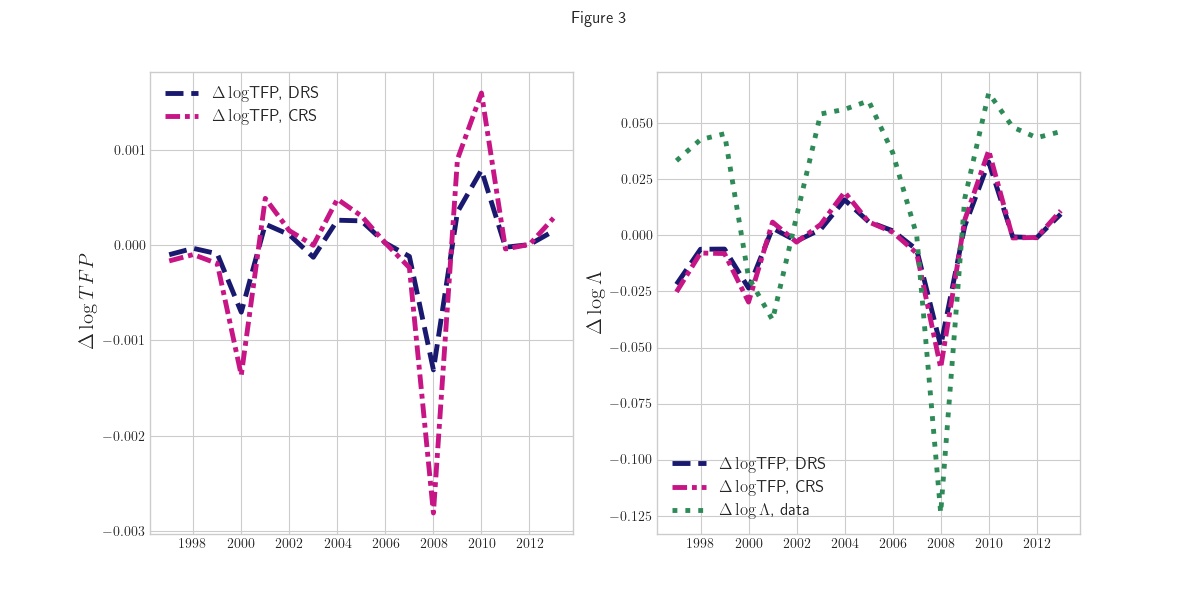
\includegraphics[scale=0.5]{figure3.png}
\caption{Model-Generated Wedges and Data Counterpart}
\label{model_wedges}
\end{figure}

\paragraph*{Decomposition of Aggregate Consumption and Labor between TFP and the Labor Wedge:}

Next, we transform the model-implied fluctuations in the two wedges into model-implied time series for aggregate consumption and labor. We report the results for this transformation in Figure \ref{decomposition}, where in the two upper panels show model-implied aggregate consumption and in the two lower panels we report model-implied aggregate labor. The left panel plots these series for the DRS model, while those for the CRS
model are plotted on the right. As suggested by theory, fluctuations in the labor wedge (colored in green) accounts for most of the fluctuations observed in aggregate consumption and labor. In particular, in the DRS model 93\% of the drop in consumption and 97\% of the fall in labor
during the recession is due to the labor wedge; the corresponding numbers in the CRS model are 96\% and 97\%.

\begin{figure}[!h]
\centering
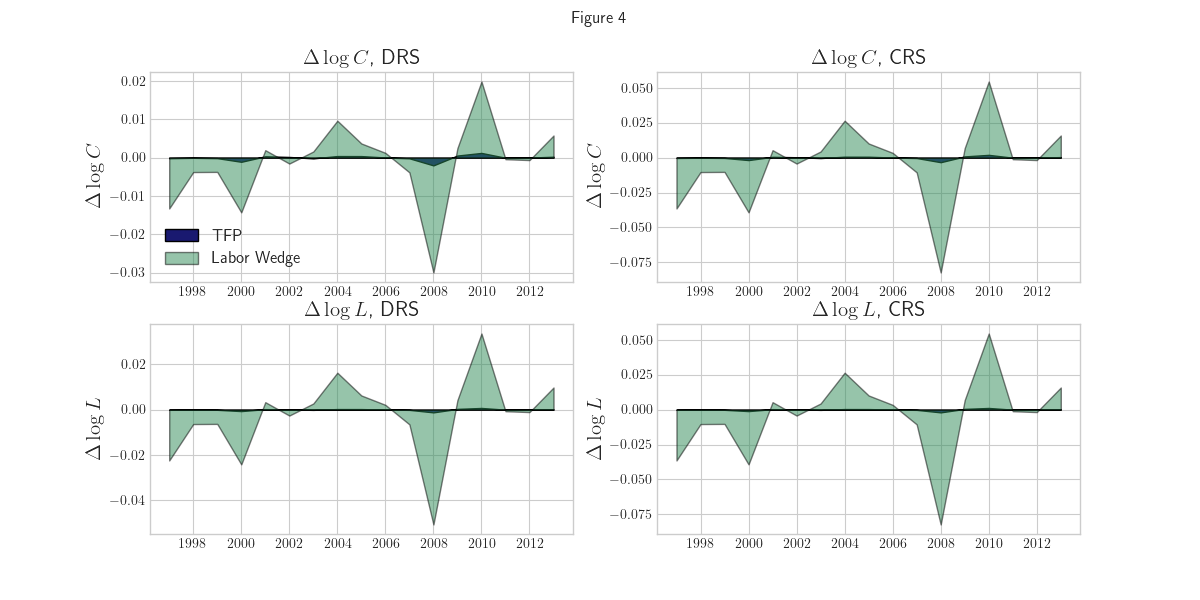
\includegraphics[scale=0.5]{figure4.png}
\caption{Decomposition of $C$ and $L$ between TFP and the Labor Wedge}
\label{decomposition}
\end{figure}


\clearpage

\section*{Proposal: Wage and Employment Fluctuations in Production Networks}

\paragraph*{Summary of Bigio and La'O QJE 2020}

This paper underlines the importance of the Input-Output production structure of the economy in amplifying the effects of micro distorsions on the aggregate fluctuations of the efficiency and labor wedges. While aggregate TFP does not strongly react to a shock in the sectoral specific cost of borrowing, the labor wedge seems to be strongly influenced by the underlying network structure of the economy, suggesting a network multiplier of $\approx 2$. This result stems from micro founded distorsions defined as:
\begin{align*}
\phi_i = \frac{1}{1 + r^{GZ}_{it}}
\end{align*}
where $r^{GZ}_{it}$ is the sector-specific intraperiod borrowing rate, as defined by \cite{gilchrist2012credit}. 

One of the main contribution to the existing literature is the introduction of an elastic labor supply decision by the household, which allows the financial friction on the production side to generate distortions at aggregate level. Therefore, the assumptions modelling for the household labor supply decision, has important consequences for understanding how the financial frictions on the supply side propagates to the whole economy. 

In this paper, the household decides the optimal aggregate labor supply $L(s)$. Labor demand $\ell_{i,k}(s)$ from each different sector $i$ is determined by the intermediate firms' optimal input decisions. The characterization of the equilibrium requires that the resource constraints is always satisfied with equality \textit{i.e.} $L(s) = \sum_{i \in I} \ell_i(s)$. This implies that labor is perfectly mobile between sectors, so that when financial shocks hit sectors differently, they can perfectly adjust the labor demand and, similarly, the household can perfectly adjust the labor supply. In this setup, aggregate wages move to ensure that labor supply is always equal to labor demand.


\subsection*{Motivation}

I propose to study wage and employment fluctuations in an economy that features heterogeneity in human capital on the household side and production networks on the production side. Using the same definition of financial frictions as in \cite{bigio2020distortions}, I could study whether financial frictions can be responsible for employment and wage fluctuations when labor demand for different occupations is different across sectors, and each sector is subject to a different \textit{intraperiod borrowing rate} to finance its working capital. Heterogeneity in human capital drives occupational choice by the household and the input-output structure of the economy impact sectoral demand for different occupations. By feeding the same \cite{gilchrist2012credit} excess bond premia, I could quantify whether these financial frictions are responsible for wage and employment fluctuations, and whether the mechanism and the model are relevant to match the observed movement of wages and employment observed during the Great Recession.


\subsection*{Possible Framework} 

In the framework I propose, households are indifferent between sectors, conditional on the occupation they choose. They can optimally decide in which occupation to work, being subject to stochastic costs of maintaining human capital and taste shocks per occupation. 

Workers can now optimally choose in which occupation to work. For tractability, I assume that human capital is unidimensional, but individuals can accumulate human capital differently depending on the occupation they choose. The law of motion for human capital is defined as $h_{it+1} = g \left( h_{it},\eta(o_t) \right)$ where $h_{it}$ is the human capital of individual $i$ at time $t$ and $\eta \left( o_t \right)$ is an occupation specific shock to human capital. Human capital evolves randomly according to the stochastic component $\eta \left( o_t \right)$ which is larger for occupation whose tasks allows the individual to increase knowledge and skills\footnote{A limitation of this approach is due to the fact that I am ignoring multidimensional human capital. For example, an individual can potentially have large shocks to human capital in any occupation \textit{i.e.} a construction site workers could improve a lot in the job he is performing. The interpretation of human capital in this model is strictly related to how wage are defined for different individuals: if you accumulate more skills in certain occupation it does not necessarily mean that your wage will increase because you are more skilled in that occupation \textit{i.e.} construction site workers' wages do not increase over time cause they become more skilled at performing that job.}. 

\paragraph*{Household}
Following \cite{grigsby2022skill}, I assume that there exists a continuum of workers with mass one, where each workers can supply a specific amount of human capital. There is a unitary household with the whole mass one workers that consume an aggregated good $C$. These workers can choose in which of the $O$ occupation to work, where $0\in O$ gives the opportunity to the household to remain unemployed. Workers are hand-to-mouth, so they consume their wage $w_t (o_t)$ which depends on the occupation they choose, and gain utility $u(\cdot)$ from consumption. In each period, workers are subject to a cost of maintaining human capital $C\left( h_{it}, \xi \left( o_{t-1} \right) \right)$ which is a function of their level of human capital $h_{it}$ and of a random shock $\xi \left( o_{t-1} \right)$ whose distribution changes depending on the occupation in which they have been employed.


Finally, worker $i$ chooses in which occupation $o$ to work in order to maximize his lifetime utility\footnote{I assume that the household problem is stationary.}:
\begin{align}
\begin{split}
  V(h_{it},o_{t-1}) &= \max\limits_{o_t \in \{0,1,\ldots,O\}} \ u\left( h_{it} w_t (o_t) \right) - C\left( h_{it}, \xi \left( o_{t-1} \right) \right) + \zeta_{iot} + \beta \mathbb{E} \left[ V\left(h_{it+1} | o_t \right) \right] \\
  h_{it+1} &= g \left( h_{it},\eta(o_t) \right)
\end{split}
\end{align}
where $\zeta_{iot}$ is an individual-occupation specific taste shock.

Assuming that $\zeta_{iot}$ has an Extreme Value Type 1 distribution with scale $\nu \left( o_t \right)$ we can write the aggregate labor supply per occupation as:
\begin{align}
L^{o}_t\left( \mathbf{w_t} \right) = \frac{\exp\left( \frac{ u\left( h_{it} w_t (o_t) \right) - C\left( h_{it}, \xi \left( o_{t-1} \right) \right) +  \beta \mathbb{E} \left[ V\left(g \left( h_{it},\eta(o_t) \right) | o_t \right) \right]  }{\nu \left(o_t \right)}\right)}{\sum_{o_t' \in {0,1,\ldots,O}} \exp\left( \frac{ u\left( h_{it} w_t (o'_t) \right) - C\left( h_{it},\xi \left( o_{t-1} \right)  \right) + \beta \mathbb{E} \left[ V\left(g \left( h_{it},\eta(o'_t) \right)  \right) \right]   }{\nu \left(o_t \right) }\right)}
\end{align}


\paragraph*{Production}
On the production side, I follow \cite{bigio2020distortions} and assume that the economy has an Input-Output structure, made of $I$ different sectors, each with a representative firm that produces an intermediate good that is then aggregate by a monopolist producer. This monopolist producer is a representative competitive firm which produces numeraire using the output from the set $I$ of intermediate goods sectors as inputs to a constant elasticity of substitution (CES) production function. Differently from \cite{bigio2020distortions}, and similarly to \cite{grigsby2022skill}, I assume that now the firms can also employ different type of labor\footnote{I omit the time subscript to ease the notation.}:
\begin{align*}
y_{i} &= z_i F_i (\ell_{i}, x_{i}) \\
x_{i} &\equiv G_i \left( \boldsymbol{x_i} \right) \\
\textcolor{violet}{\ell_{i}} &\equiv \textcolor{violet}{H_i \left( \boldsymbol{\ell_{i}} \right)}
\end{align*}
where $\boldsymbol{x_i} = \left( x_{i1},\ldots,x_{iI} \right)$ is the amount of good purchased from each sector by sector $i$ and $\boldsymbol{\ell_{i}} = \left( \ell_{i1},\ldots, \ell_{iO} \right)$ is the amount of labor of type $o$ employed in sector $i$. The profits of the representative firm in sector $i$ are equal to:
\begin{align*}
\pi_{i} = p_{i} y_{i} - \textcolor{violet}{\sum_{o \in O} w_{o} \ell_{io}} - \sum_{j \in I} p_j x_{ij}
\end{align*}
where $p_{i}$ is the price at which it sells its own input and $w_o$ is the cost of type $o$ labor.

\begin{comment}

\paragraph*{Timing Assumption for the household decision problem} 
We assume that the individual decision is divided in two stages. In the first stage an individual must decide whether to work or being unemployed:
\begin{align*}
  V(h_{it}) &= \max \Big\{  V(h_{it})^E, V(h_{it})^U \Big\} 
\end{align*}
where $V(h_{it})^U$ is the value of being unemployed:
\begin{align*}
  V(h_{it})^U &= b - C(0) + \zeta_{i0t} + \beta \mathbb{E} \left[ V(h_{it+1}) \right] \\
  h_{it+1} &= h_{it} - \eta_{it}(0)
\end{align*}
where$b$ are unemployment benefits, $C(0)$ is the unemployment specific shock and the law of motion for capital is decreasing in $\eta_{it} (0)$\footnote{The interpretation here is that human capital depreciates as the individual remains unemployed.}. 

$V(h_{it})^E$ is the expected value of being employed in period $t$:
\begin{align*}
  V^E(h_{it}) &= \max\limits_{o_t \in \{0,1,\ldots,O\}} \ u\left( h_{it} w_t (o_t) \right) - \mathbb{E}_{\xi} \left[ C\left( h_{it}, \xi \left( o_{t} \right) \right]\right) + \beta \mathbb{E} \left[ V^o(h_{it}) \right] 
\end{align*}
In the second stage, costs of maintaining human capital realize and the worker must choose in which occupation to work, being subject to an occupation specific taste shock:
\begin{align*}
  V^o(h_{it}) &= \max\limits_{o_t \in \{0,1,\ldots,O\}} \ u\left( h_{it} w_t (o_t) \right) - C\left( h_{it}, \xi \left( o_{t} \right) \right) + \zeta_{iot} + \beta \mathbb{E} \left[ V\left(h_{it+1} \right) \right] \\
  h_{it+1} &= g \left( h_{it},\eta(o_t) \right)
\end{align*}


\paragraph*{Example - Cobb-Douglas Economy with Linear Preference and Cost}
\begin{align*}
F_i (\ell_i, x_i) &= \ell^{\alpha_i} {x_i}^{1-\alpha} \\
G_i \left( \boldsymbol{x_i} \right) &= \prod_{j \in I} x_{ij}^{g_{ij}} \\
H_i \left( \boldsymbol{\ell_{i}} \right) &= \prod_{j=1}^K \ell_{ij}^{\theta_{ij}}
\end{align*}

\end{comment}

\paragraph*{Equilibrium and Solution Method} To properly derive an equilibrium in this economy I would need to work out the algebra a bit more, but here I provide a general sketch of what this equilibrium would look like. The equilibrium in this economy requires that:
\begin{enumerate}
	\item The workers' occupation choice is optimal;
	\item Intermediate goods producers first-order conditions are satisfied;
	\item The monopolist's demand for each sector output is equal to the output produced by the representative firm in each sector $i$;
	\item Final aggregated goods market clears, that is $Y = C = I + \Pi$;
	\item Labor-markets for each occupation clear:
	\begin{align*}
		L^{o}_t\left( \mathbf{w_t} \right) &= \sum_{i = 1}^I \ell_{io}
	\end{align*}
\end{enumerate}

My idea is to follow \cite{rust1987optimal} to model the dynamic decision problem of the workers and use a similar solution method to estimate/calibrate the labor supply parameters. The absence of aggregate shocks in this framework would relatively simplify the solution of the model.


\clearpage

\bibliographystyle{abbrvnat}
\bibliography{references.bib}

\end{document}

